%
% related-work.tex
%
% Copyright (C) 2022 by Universidade Federal de Santa Catarina.
%
% GNSS Networks Based on Small Satellites
%
% This work is licensed under the Creative Commons Attribution-ShareAlike 4.0
% International License. To view a copy of this license,
% visit http://creativecommons.org/licenses/by-sa/4.0/.
%

%
% \brief Related works section.
%
% \author Gabriel Mariano Marcelino <gabriel.mm8@gmail.com>
%
% \version 0.0.0
%
% \date 2021/06/14
%


\chapter{Related Work} \label{ch:related-work}

Este capítulo apresenta um resumo dos principais trabalhos relacionados e a situação atual das redes de GNSS no mundo, apresentando-se o histórico e status das redes atualmente em operação, e projetos atualmente em andamento e que possivelmente serão implementados ou entraram em operação no futuro, tanto com a utilização de satélites convencionais quanto com satélites de pequeno porte.

\section{Current GNSS networks}

Atualmente existem quatro redes de GNSS em operação: GPS\nomenclature{\textbf{GPS}}{Global Positioning System}, GLONASS\nomenclature{\textbf{GLONASS}}{\textit{Globalnaya navigatsionnaya sputnikovaya sistema}}, Galileo e BDS\nomenclature{\textbf{BDS}}{BeiDou Navigation Satellite System}. Além de mais duas redes locais, que operam de forma limitada a uma região específica: QZSS\nomenclature{\textbf{QZSS}}{Quasi-Zenith Satellite System} e IRNSS\nomenclature{\textbf{IRNSS}}{Indian Regional Navigation Satellite System}.

Abaixo, encontra-se uma descrição de cada uma dessas redes.

\subsection{GPS}

O GPS \cite{gps}, ou Global Positioning System, é o sistema de GNSS desenvolvido e mantido pelos Estados Unidos. Foi o primeiro sistema de navegação global por satélite a ser desenvolvido e entrar em operação, tendo o projeto sido iniciado em 19XX e os primeiros satélites lançados em 1978. A rede se tornou operacional em 1995 e teve custo total de 10 bilhões de dólares. Atualmente possuí 24 satélites em operação, operando a uma altitude de aproximadamente 20200 quilômetros e com a premissa de se ter sempre pelo menos quatro satélites cobrindo qualquer ponto do planeta.

Atualmente o sistema é de uso civil e militar, mas até a década de 2000, o sistema possuía precisão propositalmente limitada para dispositivos de uso civil, sendo seu uso em capacidade máxima destinado somente a aplicações militares. Por questões de segurança, erros propositais eram induzidos aos sinais transmitidos de forma que receptores de uso geral não possuíssem precisão menor que 90 metros.


\subsection{GLONASS}

O GLONASS, sigla de \textit{Globalnaya navigatsionnaya sputnikovaya sistema} (ou Sistema de Navegação Global por Satélite) \cite{glonass}, é o sistema de GNSS criado e mantido pela Rússia.

GLONASS (Globalnaya Navigazionnaya Sputnikovaya Sistema, or Global Navigation Satellite System) is a global GNSS owned and operated by the Russian Federation. The fully operational system consists of 24+ satellites.

\subsection{Galileo}

O Galileo é o sistema de GNSS criado pela união europeia.

Galileo is a global GNSS owned and operated by the European Union. The EU declared the start of Galileo Initial Services in 2016 and plans to complete the system of 24+ satellites in 2021.

\subsection{BDS}

O \textit{BeiDou Navigation Satellite System}, ou BDS \cite{beidou}, é o sistema de GNSS chinês.

BeiDou, or BDS, is a global GNSS owned and operated by the People's Republic of China. BDS was formally commissioned in 2020. The operational system consists of 35 satellites. BDS was previously called Compass.



A \autoref{tab:networks-comparison} compara as principais características dos sistemas de GNSS apresentados acima.

\begin{table*}[!h]
    \centering
    \begin{tabular}{lcccccc}
        \toprule[1.5pt]
        \multirow{2}{*}{\textbf{Characteristic}} & \multicolumn{6}{c}{\textbf{Network}} \\
                                                 & \textbf{GPS} & \textbf{GLONASS} & \textbf{Galileo} & \textbf{BDS} & \textbf{QZSS} & \textbf{IRNSS} \\
        \midrule
        Coverage                         & Global            & Global                       & Global               & Global         & Local   & Local \\
        Country                          & United States     & Russia                       & European Union       & China          & Japan   & India \\
        Satellites                       & 32                & 24                           & 30                   & 30             &         &  \\
        Orbit                            &                   &                              &                      &                &         &  \\
        Altitude                         &                   &                              &                      &                &         &  \\
        \multirow{6}{*}{Frequency [MHz]} & 1575,42           & 1598,0625-1609,3125          & 1575,42              & 1561,098       & 1575,42 & 1176,45 \\
                                         & 1227,6            & 1242,9375-1251,6875          & 1176,45              & 1207,14        & 1227,6  &  \\
                                         & 1176,45           & 1202,025                     & 1207,14              & 1268,52        & 1176,45 &  \\
                                         &                   &                              & 1191,795             & 1575,42        & 1278,75 &  \\
                                         &                   &                              & 1275,75              & 1176,45        &         &  \\
                                         &                   &                              &                      & 1207,14        &         &  \\
        Bandwidth [MHz]                  & 15,345/11/12,5    &                              &                      &                &         &  \\
        Modulation                       &                   &                              &                      &                &         &  \\
        Precision                        &                   &                              &                      &                &         &  \\
        Status                           & Fully operational &                              &                      &                &         &  \\
        \bottomrule[1.5pt]
    \end{tabular}
    \caption{Comparison between the current operational GNSS networks.}
    \label{tab:networks-comparison}
\end{table*}

%        \multirow{6}{*}{Frequency [MHz]} & 1575,42 (L1 C/A)  & 1598,0625-1609,3125 (L1 C/A) & 1575,42 (E1)         & 1561,098 (B1l) & 1575,42 (L1 C/A/S) & 1176,45 (L5) \\
%                                         & 1227,6 (L2 C/P)   & 1242,9375-1251,6875 (L2 C/P) & 1176,45 (E5a)        & 1207,14 (B2l)  & 1227,6 (L2C)       &  \\
%                                         & 1176,45 (L5)      & 1202,025            (L3 OC)  & 1207,14 (E5b)        & 1268,52 (B3l)  & 1176,45 (L5)       &  \\
%                                         &                   &                              & 1191,795 (E5 AltBOC) & 1575,42 (B1C)  & 1278,75 (L6)       &  \\
%                                         &                   &                              & 1275,75 (E6)         & 1176,45 (B2a)  &                    &  \\
%                                         &                   &                              &                      & 1207,14 (B2b)  &                    &  \\

\section{Local networks}

.

\subsection{QZSS}

The Quasi-Zenith Satellite System \cite{qzss} (QZSS, or also know as Michibiki) is a local positioning system developed by the Japanese government covering part of Asia and Oceania, focusing primordially on the japanese territory. The objective of this system is to improve the GPS system coverage in the region with higher stability and precision. Currently, the system is composed by four satellites (QZS-1, 2, 3 and 4) and it is compatible with the GPS, but an independent system is also planned to be operational with seven satellites in 2023.

The QZSS operates with one geostationaty satellite and three in a Tundra highly inclined, slightly elliptical, geosynchronous orbit, with each satellite 120$^{\circ}$ apart from each other. quasi-zenith orbit (QZO\nomenclature{\textbf{QZO}}{Quasi-Zenith Orbit}) scheme. This orbit is illustrade in \autoref{fig:qzss-orbit}.

\begin{figure}[!ht]
    \begin{center}
        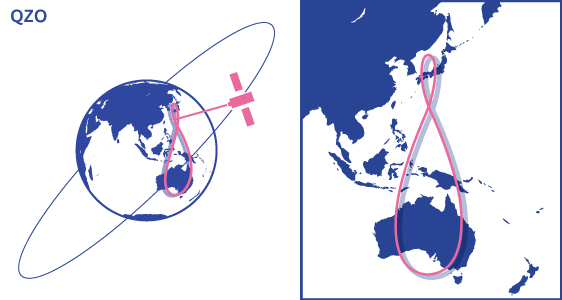
\includegraphics[width=0.8\columnwidth]{figures/qzss-orbit}
        \caption{Quasi-Zenith orbit of the QZSS network \cite{qzss}.}
        \label{fig:qzss-orbit}
    \end{center}
\end{figure}

The orbital elements of the QZSS satellites are available in \autoref{tab:qzss-orbit-config}.

\begin{table*}[!h]
    \centering
    \begin{tabular}{lc}
        \toprule[1.5pt]
        \textbf{Keplerian Elements} & \textbf{Value} \\
        \midrule
        Epoch                                   & 26 December 2009, 12:00 UTC \\
        Semimajor                               & 42164 km \\
        Eccentricity                            & $0,075 \pm 0,015$ \\
        Inclination                             & $43 \pm 4^{\circ}$ \\
        Right ascension of the ascending node   & $195^{\circ}$ \\
        Argument of perigee                     & $270 \pm 2^{\circ}$ \\
        Mean anomaly                            & $305^{\circ}$ \\
        Central longitude of ground trace       & $135\ E \pm 5^{\circ}$ \\
        \bottomrule[1.5pt]
    \end{tabular}
    \caption{Orbit configuration of the QZSS.}
    \label{tab:qzss-orbit-config}
\end{table*}

\subsection{IRNSS}

The IRNSS (Indian Regional Navigation Satellite System) \cite{irnss} is a regional and independent nagivation system developed and maintained by India, focusing on covering mainly its territory. This network is currently composed by a constellation of seven satellites, three in a geostationaty orbit, and four in a geosynchronous orbit.

IRNSS is a regional GNSS owned and operated by the Government of India. IRNSS is an autonomous system designed to cover the Indian region and 1500 km around the Indian mainland. The system consists of 7 satellites. In 2016, India renamed IRNSS as the Navigation Indian Constellation (NavIC, meaning ``sailor'' or ``navigator'').

\begin{figure}[!ht]
    \begin{center}
        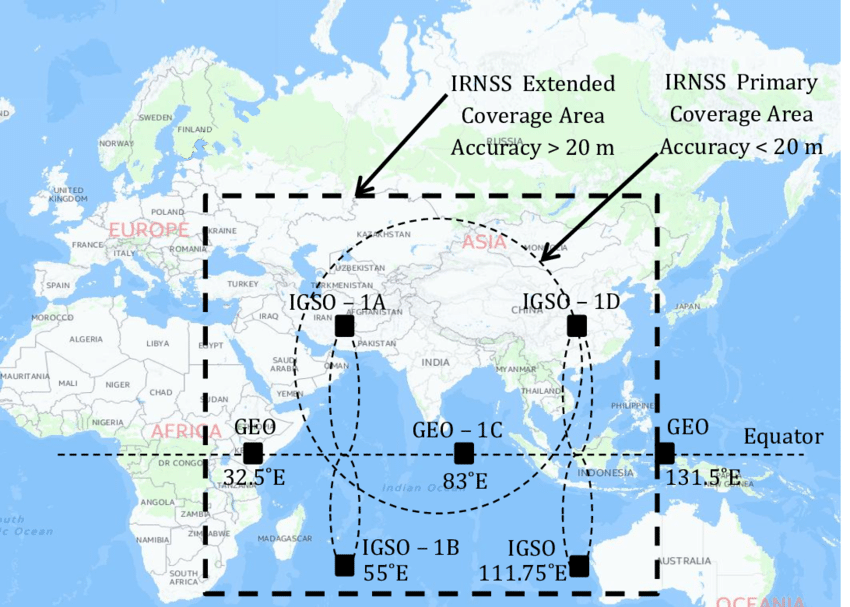
\includegraphics[width=0.8\columnwidth]{figures/irnss}
        \caption{IRNSS satellites and coverage (adapted from \cite{thombre2015}).}
        \label{fig:irnss}
    \end{center}
\end{figure}

\section{Experimental GNSS networks}

Recentemente, com o avanço dos nanossatélites, o crescimento de dispositivos com conectividade e a Internet das coisas (IoT), começou a surgir ideias de implantação de redes privadas e em baixa órbita de sistemas de GNSS, seja para atender propósitos específicos ou de uso geral. Considerando, começam a surgir iniciativas de empresas para a utilzação de pequenos satélites para esse tipo de aplicação, o que vai de encontro a ideia principal deste trabalho.

Dentre essas iniciativas, pode-se destacar duas startups que possuem propostas similares: TrustPoint\footnote{\href{https://www.trustpointgps.com/}{https://www.trustpointgps.com/}} e Xona Space Systems\footnote{\href{https://www.xonaspace.com/}{https://www.xonaspace.com/}}.

A primeira tem como proposta o uso 

Já a segunda \cite{aarestad2020}, propõe a implantação de redes privadas de GNSS, utilizando satélites em baixa órbita. Uma imagem conceitual de um dos satélites da rede pode ser vista na \autoref{fig:xona-satellite}.

\begin{figure}[!ht]
    \begin{center}
        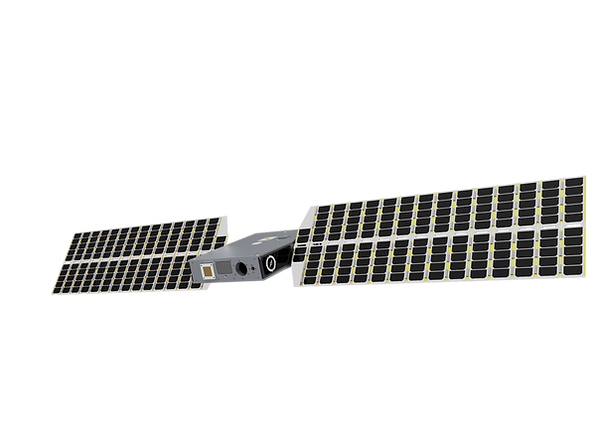
\includegraphics[width=0.8\columnwidth]{figures/xona-satellite}
        \caption{Xona Space Systems conceptual satellite.}
        \label{fig:xona-satellite}
    \end{center}
\end{figure}

\section{Remarks}

Até o momento, não se conhece outras teses de doutorado sobre este tema. Como apresentado acima, já existem iniciatis comerciais que visam implantar redes de GNSS privadas utilizando pequenos satélites, mas não há nenhuma rede totalmente operacional até o momento.
